\subsection{ChanceController}
\begin{figure}[H]
    \centering
    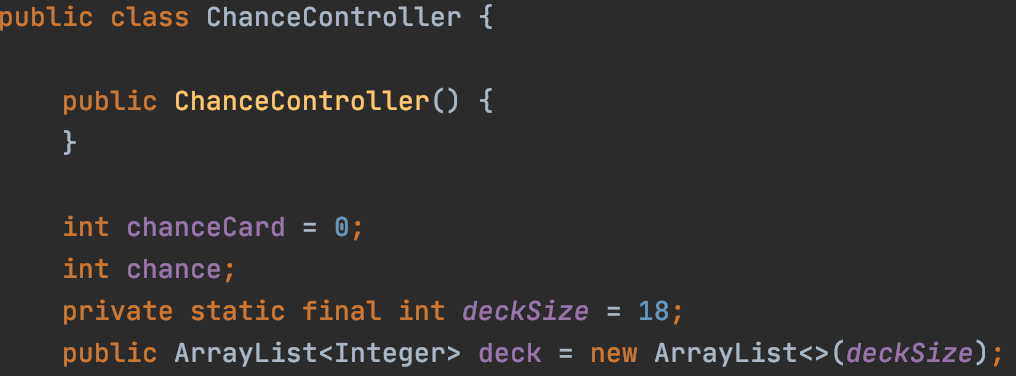
\includegraphics{sources/7_implementering/ControllerClass.png}
    \caption{Vores variable i ChanceController klassen}
    \label{fig:ChanceController}
\end{figure}
I ChanceController klassen har vi to integers, chanceCard og chance. Vores final int deckSize bruger vi til vores chancekort, som vi danner en bunke af ved hjælpe af vores ArrayList.




\begin{figure}[H]
    \centering
    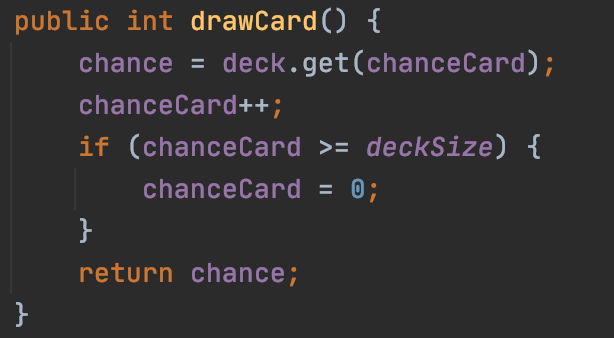
\includegraphics{sources/7_implementering/ControllerDraw.png}
    \caption{Metode til at trække et chancekort}
    \label{fig:draw}
\end{figure}
drawCard metoden bruges til at trække det øverste kort i vores bunke, som vi lavede med ArrayList. Dette fortsætter indtil chance-nummeret bliver lige så højt som vores deckSize, da dette angiver vores kortbunke. Når vi når bunden af bunken, starter den forfra osv.





\begin{figure}[H]
    \centering
    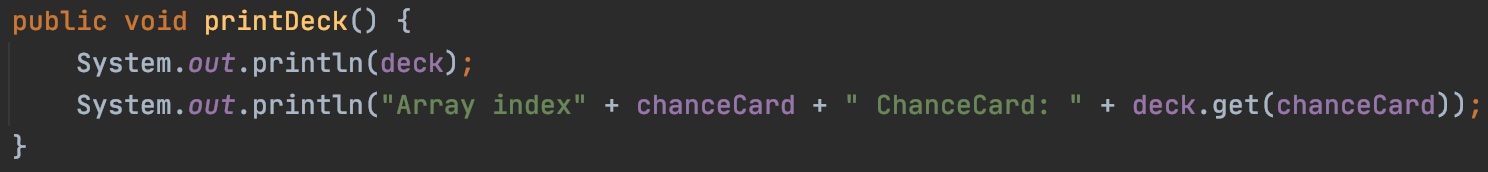
\includegraphics[width=0.7\textwidth]{sources/7_implementering/ControllerprintDeck.png}
    \caption{Metode til at printe dækket og holde styr på bunken}
    \label{fig:print}
\end{figure}
printDeck metoden printer vores dæk i terminalen. Når et nyt chancekort bliver trukket, printer den i terminalen hvilket nummer i arrayet, der blev trukket, og hvilket chancekort (i case rækkefølgen) dette kort er.




\begin{figure}[H]
    \centering
    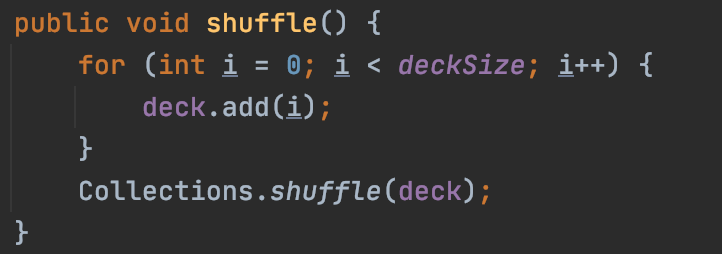
\includegraphics{sources/7_implementering/Controllershuffle.png}
    \caption{Når kortene i bunken skal blandes}
    \label{fig:shuffle}
\end{figure}
Shuffle metoden blander vores chancekort i en tilfældig rækkefølge og danner dermed en bunke.



\begin{figure}[H]
    \centering
    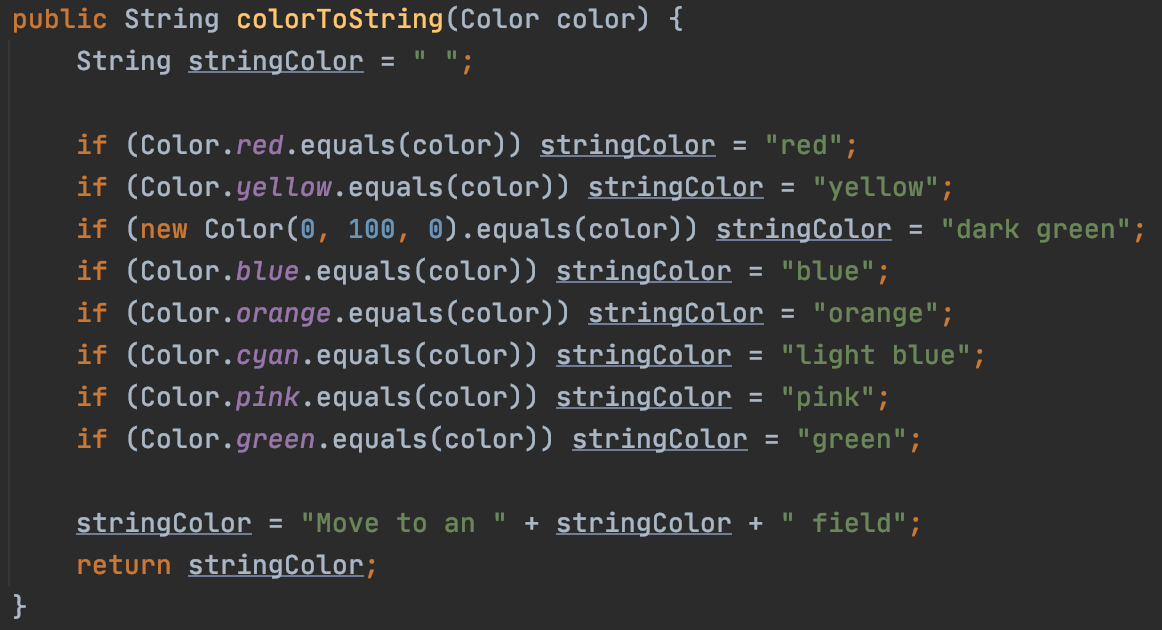
\includegraphics[width=0.7\textwidth]{sources/7_implementering/ControllercolortoString.png}
    \caption{Omdan strings til farve}
    \label{fig:colorString}
\end{figure}
stringColor metoden bruges til at danne strings af alle de farver, som de forskellige felter kan have. Alt efter hvilken farve, man skal lande på, bliver det skrevet på en string.



\begin{figure}[H]
    \centering
    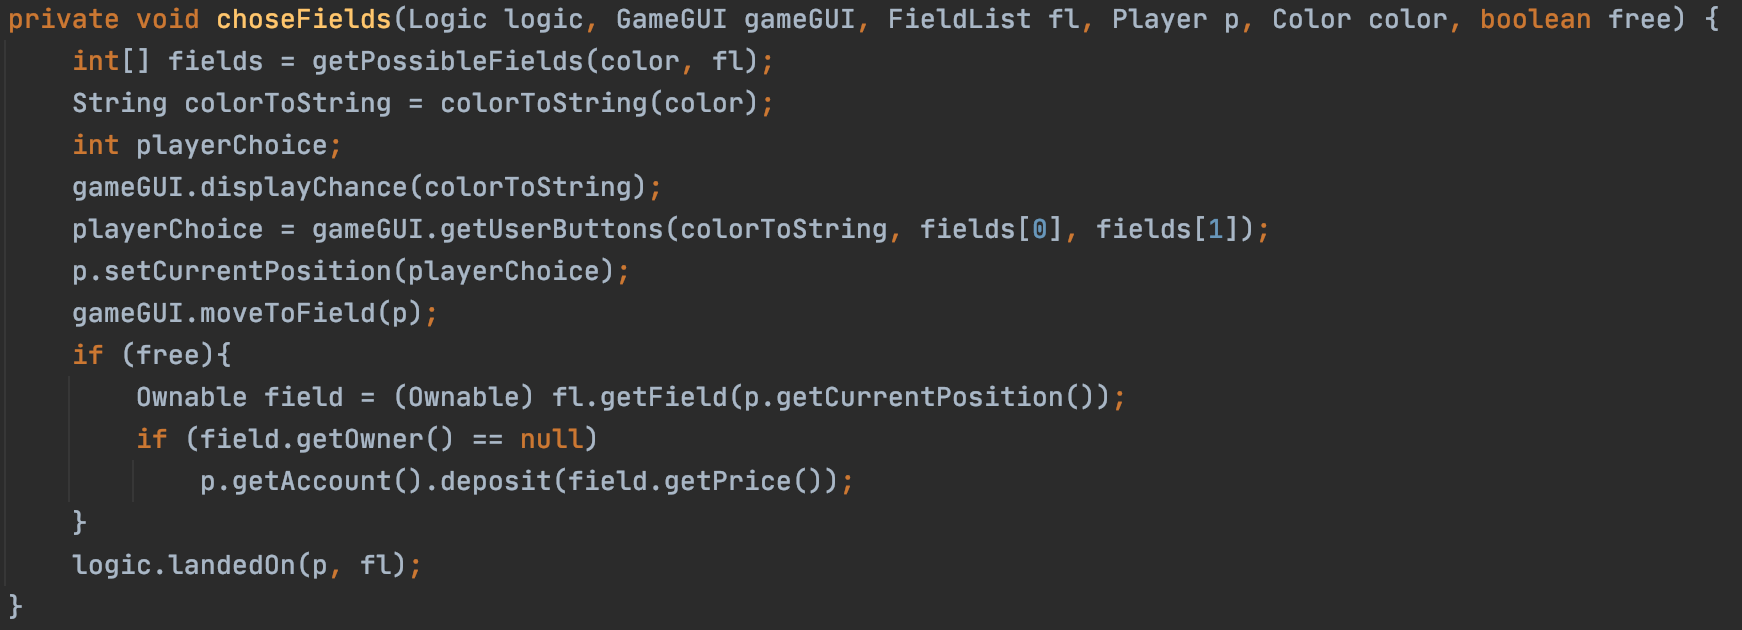
\includegraphics[width=0.7\textwidth]{sources/7_implementering/ControllerchooseFields.png}
    \caption{Vælg et felt af en bestemt farve, man vil rykke til}
    \label{fig:chooseFields}
\end{figure}
chooseFields metoden bruger vi til at vælge et felt, som man vil flytte til. Dette sker i de chance kort, hvor man kan flytte til et felt med en bestemt farve. Metoden holder ligeledes øje med, om feltet er ejet eller frit, da man i så fald skal betale eller købe feltet, man lander på. Metoden sørger også for, at vise dette i GUI’en med displayChance metoden.



\begin{figure}[H]
    \centering
    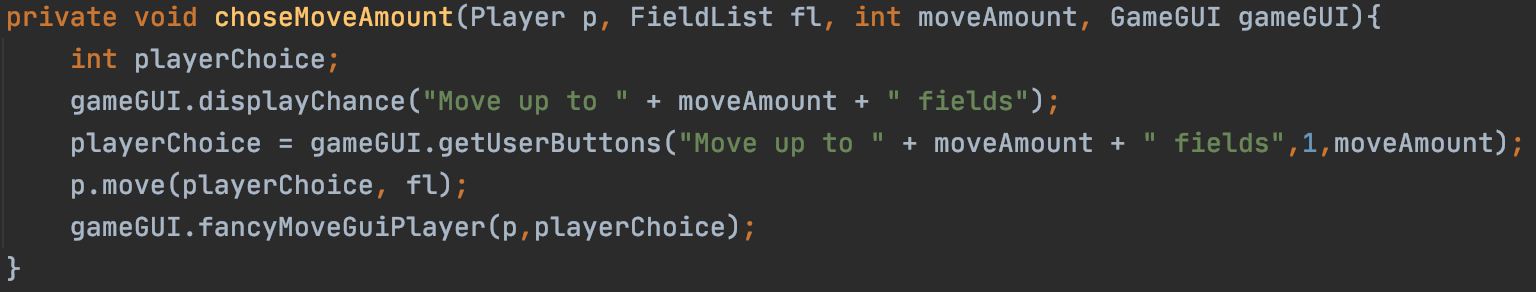
\includegraphics[width=0.7\textwidth]{sources/7_implementering/ControllerMoveAmount.png}
    \caption{Metode til at vælge antal skridt man vil tage}
    \label{fig:MoveAmount}
\end{figure}
chooseMoveAmount metoden bruges til at vælge hvor mange skridt, man vil tage, op til moveAmount. Altså kan spilleren, hvis moveAmount er 10, vælge at rykke ét til 10 felter frem.



\begin{figure}[H]
    \centering
    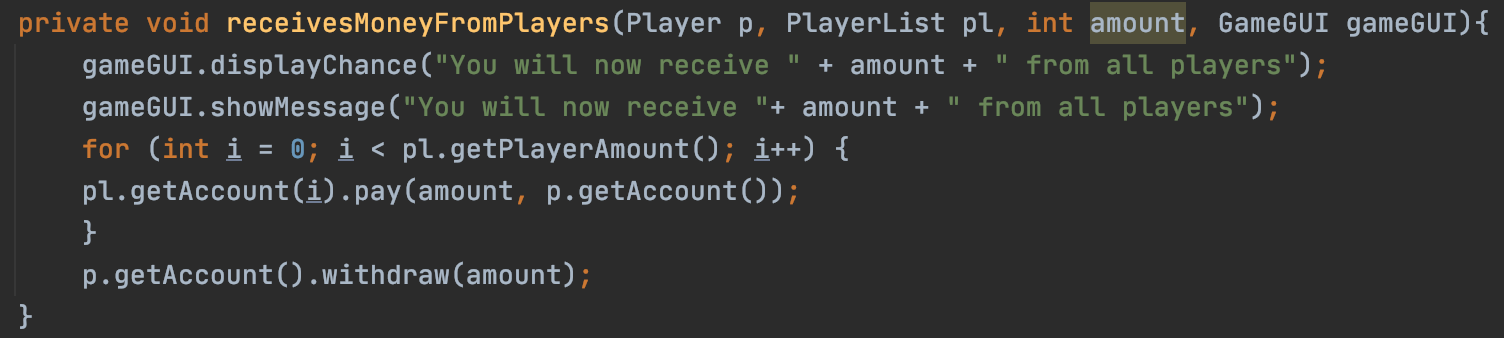
\includegraphics[width=0.7\textwidth]{sources/7_implementering/ControllerRecieveMoney.png}
    \caption{Hvis en spiller skal modtage penge fra andre spilleres konti}
    \label{fig:recieveMoney}
\end{figure}
Denne metode gør, at en spiller modtager penge fra alle andre spillere. Det sker ved, at loopet kører gennem alle spillere, som så får frataget  en bestemt mængde penge, som den éne spiller modtager.



\begin{figure}[H]
    \centering
    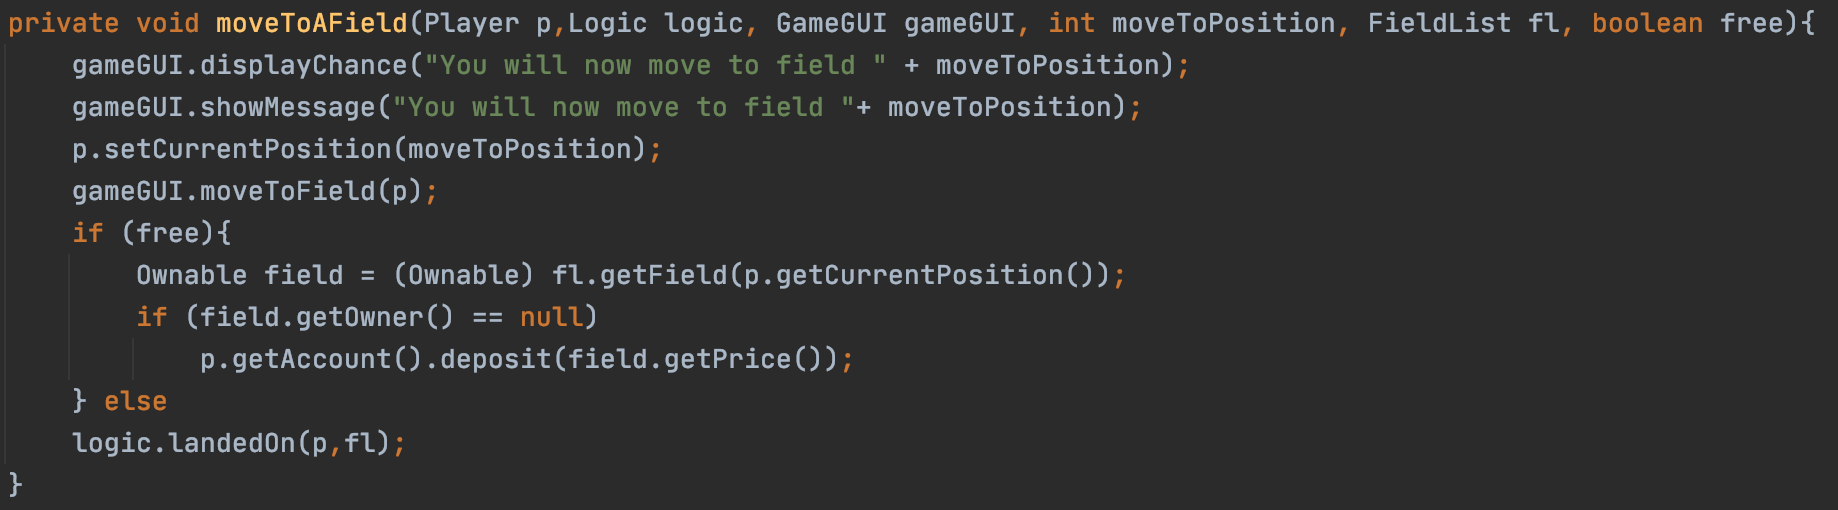
\includegraphics[width=0.7\textwidth]{sources/7_implementering/ControllermoveToField.png}
    \caption{Hvis spilleren skal bevæge sig til et bestemt felt}
    \label{fig:chance}
\end{figure}
I metoden her, bliver spilleren flyttet til et bestemt feltnummer. Når spilleren lander på feltet, tjekker metoden, om feltet kan købes og i så fald, om det er ledigt eller ej.



\begin{figure}[H]
    \centering
    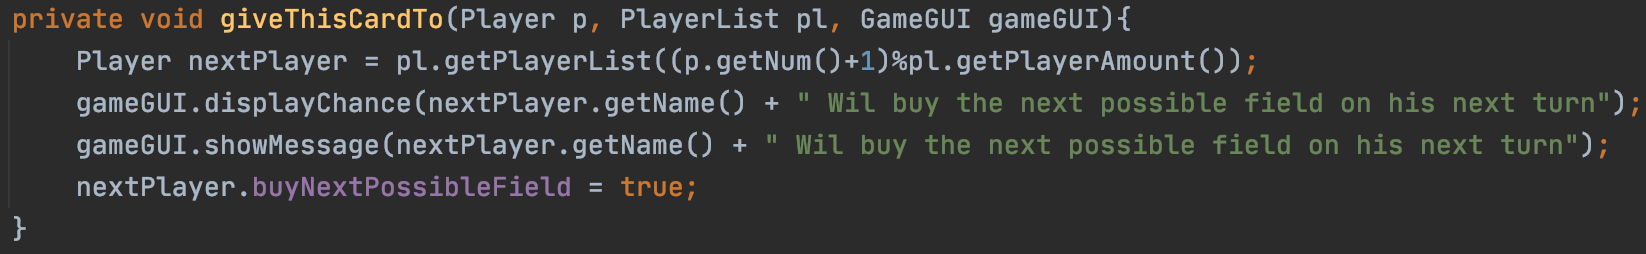
\includegraphics[width=0.7\textwidth]{sources/7_implementering/ControllerGiveCard.png}
    \caption{Metode til at give et kort til en den næste spiller}
    \label{fig:giveCard}
\end{figure}
giveThisCardTo giver et chancekort videre til den spiller, som har næste tur. Denne spiller køber det næste felt, som er ledigt. Dette sker ved buyNextPossibleField metoden.





\begin{figure}[H]
    \centering
    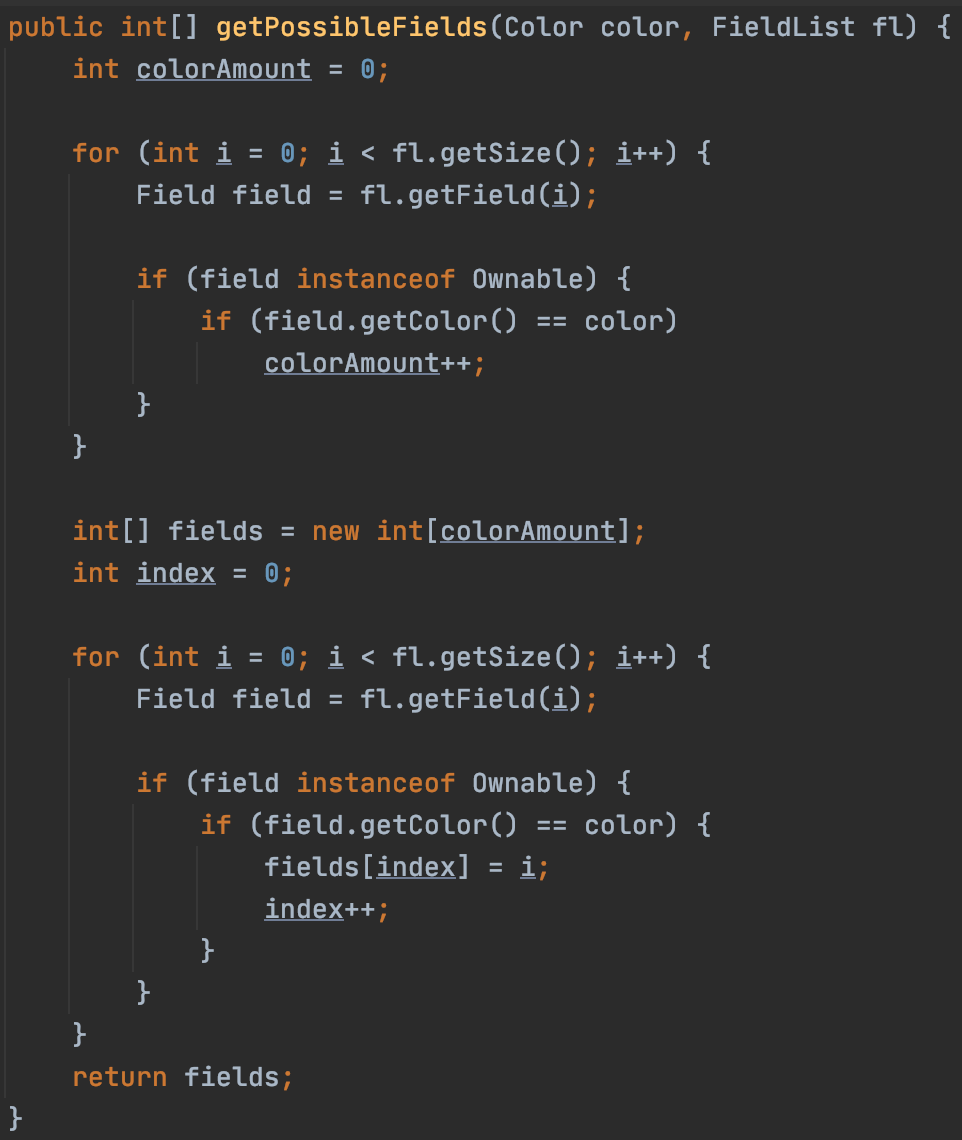
\includegraphics{sources/7_implementering/ControllerGetFields.png}
    \caption{Metode til at se felter af forskellig farve}
    \label{fig:possibleFields}
\end{figure}
Denne metode tjekker hvilke felter, der er af de forskellige farver. Den bruges i chooseFields metoden, når en spiller skal vælge et felt af en speciel farve, som de vil lande på.


\begin{figure}[H]
    \centering
    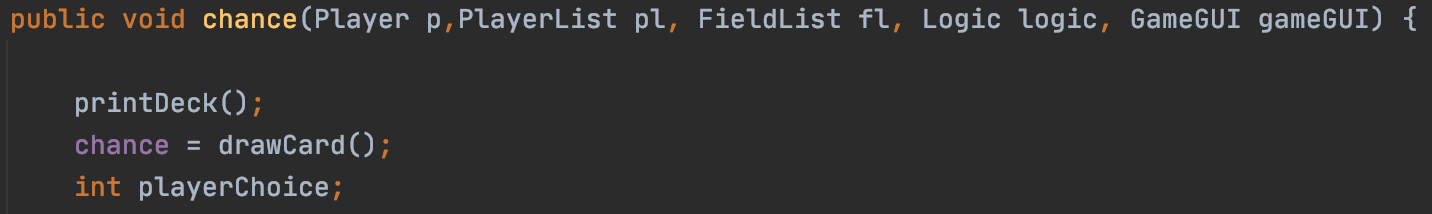
\includegraphics[width=0.7\textwidth]{sources/7_implementering/ControllerChance.png}
    \caption{Metode, som printer dæk og trækker kort når man lander på chancefelt}
    \label{fig:controllerChance}
\end{figure}

chance metoden printer dækket og trækker et kort for en spiller. Denne metode kaldes, når en spiller lander på et chancefelt. 

\begin{figure}[H]
    \centering
    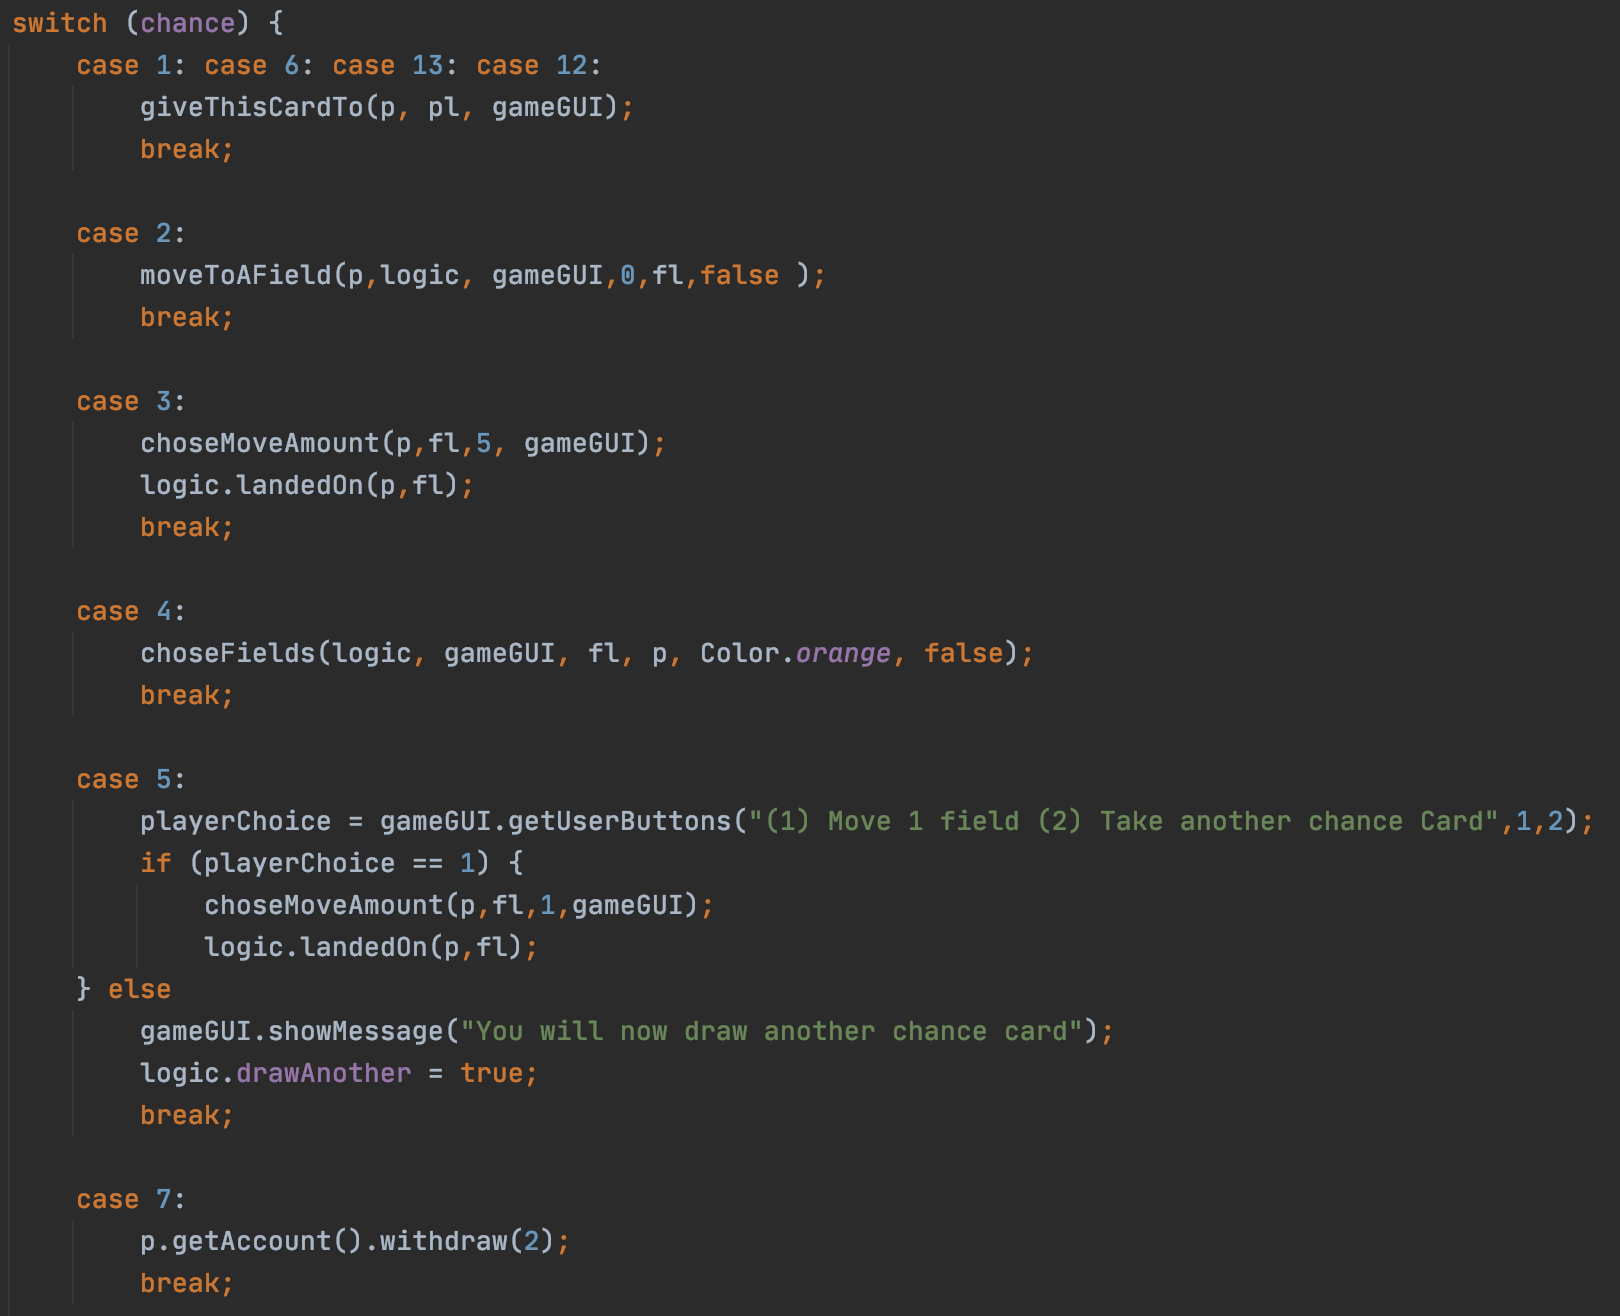
\includegraphics[width=0.7\textwidth]{sources/7_implementering/ControllerChanceSwitch.png}
    \caption{Switch-case til chancekort}
    \label{fig:ControllerChanceSwitch}
\end{figure}
Til slut har vi en længere switch-case, som repræsenterer de forskellige chancekort, som er blevet implementeret. Der er i alt 18 chancekort.












